\documentclass[10pt,a4paper,oneside, reqno]{amsproc}
\usepackage{changepage}
\usepackage{mathtext} % русские буквы в формулах
\usepackage[T2A]{fontenc}
\usepackage[utf8x]{inputenc}
\usepackage{ucs}
\usepackage{cmap}
\usepackage[english,russian]{babel}
\usepackage{graphicx}
%\usepackage{concrete}
%\usepackage{amsmath}
%\usepackage{amsfonts}
\usepackage{amssymb}
\usepackage{dcolumn}
\usepackage{booktabs}
\usepackage{ctable}
\usepackage{multirow}

\newcommand{\specialcell}[2][c]{%
  \begin{tabular}[#1]{@{}c@{}}#2\end{tabular}}
\oddsidemargin = 0pt
\textwidth = 14 cm
\topmargin = -2 cm
\textheight = 24 cm
\makeatletter
\renewcommand{\theequation}{\thesection.\arabic{equation}}
\@addtoreset{equation}{section}
\newcommand{\eq}{\begin{equation}}
\newcommand{\eeq}{\end{equation}}
\newcommand{\fr}{\frac}
\newcommand{\mf}{\mathfrak}
\newcommand{\sub}{\subsection}
\newcommand{\subsub}{\subsubsection}
\newcommand{\definition}{\theoremstyle{definition}}
\newcommand{\mult}[2]{\genfrac{\left[}{\right.}{0pt}{}{#1}{#2}}
\renewcommand{\qed}{\begin{center} $\mathsf{QED}$ \end{center}}
\newcommand{\al}{\alpha}
\newcommand{\comment}[1]{\marginpar{\Small{{\sl #1}}} }
\newcommand{\epigraph}[2]{\begin{flushright} {\em #1}\\#2\\[20 pt]
\end{flushright}}
\newcommand{\fx}[1]{\ensuremath{\mathit{f}_{#1}(x)}}
\newcommand{\re}[1]{(\ref{#1})}
\newcommand{\mh}{\mathit}
\newcommand{\itm}[1]{\begin{itemize}	\item #1 \end{itemize}}
\newcommand{\note}[1]{\begin{flushleft}\hbox{%
\vrule\hspace{.5em}\parbox{ .9\textwidth}%
{ #1}} \end{flushleft}}
\newcommand{\Al}{\ensuremath{\mathcal{A}}}
\newcommand{\@dotsep}{3.9}
\newcommand{\system}[1]{\eq\left\{ \begin{aligned} #1
\end{aligned}\right.\\[5 pt]\eeq}
\renewcommand{\phi}{\varphi}

% http://www.texnik.de/floats/caption.phtml
% This does spacing around caption.
%\setlength{\abovecaptionskip}{6pt}   % 0.5cm as an example
%\setlength{\belowcaptionskip}{9pt}   % 0.5cm as an example

%%%%%%%%%%%%%%%%%%%%%%%%%%%%%%%%%%%%%%%%%%%%%%%%%%%%%%%%%%%%%%%%%%%%%%%

\author{Соколовский Роман}
\begin{document}
\begin{titlepage}
    \begin{center}
        \textsc{\large Санкт-Петербургский Государственный Университет Аэрокосмического Приборостроения}\\[5cm]
        \rule{\textwidth}{1pt}\\
        \vspace{10pt}
        { \huge \bfseries Исследование Дифракции \\[0.2cm]
        Электромагнитных Волн}\\[0.4cm]
        \hrule
        \vspace{0.4cm}
        \textsc{ {\large Отчет по Лабораторной работе №3}}
        
        \vspace{2.5cm}
        \begin{flushright}
        \begin{minipage}{0.5\textwidth}
            \begin{flushright} 
                \textsc{\small Выполнил}:\\
                \large
                Студент факультета №\textbf{5}\\
                Группы \textbf{$5025$} кафедры \textbf{52}\\[2pt]
                \textsc{Соколовский} \textsc{Р}оман \textsc{А}лександрович
            \end{flushright}
        \end{minipage}
        \end{flushright}
        \vfill
        {\large Санкт-Петербург\\2012}
    \end{center}
\end{titlepage}
\section{Цель Работы}
\begin{enumerate}
    \item Изучить основные понятия, характеризующие явление дифракции.\\
    \item Изучить метод строгого решения дифракционной задачи на бесконечном идеально проводящем цилиндре.\\
    \item Изучить метод приближенного решения дифракционной задачи --- метод волновой оптики --- на примере
          отверстия в плоском проводящем экране бесконечных размеров.\\
    \item Изучить метод приближенного решения дифракционной задачи --- метод геометрической оптики --- на 
          примере бесконечного идеально проводящего цилиндра.\\
    \item Построить математическую модель процесса дифракции плоской волны на цилиндре и отверстии в экране
          и разработать программу расчёта дифрагированных полей.\\
    \item Изучить методы измерения дифрагированных полей.\\
    \item Исследовать явления дифракции электромагнитных волн на цилиндре и отверстии.
\end{enumerate}
\section{Схема экспериментальной установки}
Исследование явления дифракции на отверстии в плоском идеально проводящем экране и проводящих цилиндрах 
проводилось на установке, схема которой приведена на Рисунке \ref{fig:scheme}.
\begin{figure}[h!t]
    \includegraphics[width = \textwidth]{../manuals/5/12-cropped.jpg}
    \caption{Схема лабораторной установки}
    \label{fig:scheme}
\end{figure}
\newpage
\section{Результаты измерений и вычислений}
\subsection{Таблицы результатов измерений и вычислений}
Исходные данные и результаты их обработки сведены в таблицы \ref{tab:table1}, \ref{tab:table2} и \ref{tab:table3}.\\

Данные расчёта углов половинной мощности приведены ниже.
$$
\text{Цилиндр}
\left\{
\begin{aligned}
    d/\lambda=0.25 & ~\Rightarrow~\theta_{0.5}=0.84\\
    d/\lambda=0.50 & ~\Rightarrow~\theta_{0.5}=1.00\\
    d/\lambda=1.00 & ~\Rightarrow~\theta_{0.5}=0.89
\end{aligned}
\right.
\text{~ ~ ~ ~ Щель}
\left\{
\begin{aligned}
    d/\lambda=1.00 & ~\Rightarrow~\theta_{0.5}=1.00\\
    d/\lambda=2.00 & ~\Rightarrow~\theta_{0.5}=0.51\\
    d/\lambda=3.12 & ~\Rightarrow~\theta_{0.5}=0.32
\end{aligned}
\right.
$$
\begin{table}[h!t]
\centering
\vspace{10pt}
\begin{tabular}{cccc} \toprule %[-2.08em]
    \text{Диаметр цилиндра} & $l(100)$ & $l(150)$ & $l(200)$ \\
\midrule
0 & 50 & 36 & 22\\
8 & 30 & 22 & 13\\
16 & 21 & 14 & 12\\
32 & 12 & 10 & 9\\
\bottomrule
\end{tabular}
\caption{Величина напряженности электрического поля, дифрагированного в 
область геометрической тени цилиндра.} 
\label{tab:table1}
\end{table}

\begin{table}[h!t]
\centering
\vspace{10pt}
\begin{tabular}{cccc} \toprule %[-2.08em]
$\theta^\circ$ & $\alpha=32$mm & $\alpha=64$mm & $\alpha=100$mm \\
\midrule
0 & 4 & 23 & 24\\
5 & 5 & 25 & 21\\
10 & 6 & 28 & 15\\
15 & 6 & 29 & 6\\
20 & 7 & 14 & 3\\
25 & 9 & 11 & 3\\
30 & 6 & 4 & 3\\
35 & 5 & 2 & 4\\
40 & 3 & 1 & 2\\
45 & 2 & 1 & 1\\
\bottomrule
\end{tabular}
\caption{Дифракция ЭМВ на щели.} 
\label{tab:table2}
\end{table}
\vspace{-90pt}

\begin{table}
\newcolumntype{W}{D{.}{.}{2.3}}
\begin{adjustwidth}{-1.5cm}{}
\vspace{10pt}
\begin{tabular}{ccWWWWWWWWW} \toprule %[-2.08em]
\newcolumntype{W}{D{.}{.}{2.3}}
%\specialcell{Gain\\threshold, \%}	&	\specialcell{JLSv2,\\number of files}	&	\specialcell{JPEG-2k,\\number of files}\\
\multirow{2}*{$\theta^\circ$} & \multirow{2}*{\specialcell{Поле без пре-\\пятствий, $l_0$}} & \multicolumn{3}{c}{$d=8$mm} & \multicolumn{3}{c}{$d=16$mm} & \multicolumn{3}{c}{$d=32$mm}\\
& & \multicolumn{1}{c}{$l_1$} & \multicolumn{1}{c}{$\Delta_1=l_0-l_1$} &
\multicolumn{1}{c}{$\Delta_{1n}$} & 
\multicolumn{1}{c}{$l_2$} & \multicolumn{1}{c}{$\Delta_2=l_0-l_2$} & 
\multicolumn{1}{c}{$\Delta_{2n}$} & 
\multicolumn{1}{c}{$l_3$} & \multicolumn{1}{c}{$\Delta_3=l_0-l_3$} & 
\multicolumn{1}{c}{$\Delta_{3n}$}\\
 \midrule
0.00 & 37.0 & 22.0 & 15.0 & 0.65 & 22.0 & 15.0 & 0.56 & 15.0 & 22.0 & 0.56\\
5.00 & 52.0 & 33.0 & 19.0 & 0.83 & 29.0 & 23.0 & 0.85 & 17.0 & 35.0 & 0.9\\
10.0 & 56.0 & 33.0 & 23.0 & 1.0 & 31.0 & 25.0 & 0.93 & 17.0 & 39.0 & 1.0\\
15.0 & 44.0 & 32.0 & 12.0 & 0.52 & 22.0 & 22.0 & 0.81 & 12.0 & 32.0 & 0.82\\
20.0 & 43.0 & 36.0 & 7.0 & 0.3 & 31.0 & 12.0 & 0.44 & 34.0 & 9.0 & 0.23\\
25.0 & 43.0 & 57.0 & -14.0 & -0.6 & 58.0 & -15.0 & -0.55 & 60.0 & -17.0 & -0.43\\
30.0 & 35.0 & 49.0 & -14.0 & -0.6 & 50.0 & -15.0 & -0.55 & 65.0 & -30.0 & -0.77\\
35.0 & 24.0 & 29.0 & -5.0 & -0.22 & 33.0 & -9.0 & -0.33 & 50.0 & -26.0 & -0.66\\
40.0 & 50.0 & 33.0 & 17.0 & 0.74 & 23.0 & 27.0 & 1.0 & 17.0 & 33.0 & 0.85\\
45.0 & 60.0 & 57.0 & 3.0 & 0.13 & 49.0 & 11.0 & 0.4 & 42.0 & 18.0 & 0.46\\
\bottomrule
\end{tabular}
\caption{Дифракция ЭМВ на цилиндре.} 
\end{adjustwidth}
\label{tab:table3}
\end{table}

% We need 4 more tables here!
\newpage
\subsection{Графики и рисунки}
Графический анализ экспериментальных данных представлен на рисунках \ref{fig:plot1}-\ref{fig:plot5}.\\

Рисунок \ref{fig:plot1} отражает зависимость энергии 
дифрагированной волны от удалённости точки наблюдения при различных физических размерах препятствия (в д.сл. цилиндра).
Из рисунка видно, что с увеличением диаметра цилиндра поле в области геометрической тени становится менее значительным, а изменение поля ---
менее динамичным.\\

Рисунок \ref{fig:plot2} визуализирует полученную на основе таблицы (\ref{tab:table3}) экспериментальную зависимость поля дифрагированной на цилиндре волны
от величины отклонения измерительного прибора при фиксированном расстоянии измерителя до цилиндра при различных диаметрах последнего. Наглядно продемонстрирован высокий коэффициент корреляции нормированных величин. Форма результирующих кривых подтверждает явление интерференции дифрагированных ЭМВ.\\

Рисунок \ref{fig:plot3} является демонстрацией аналогичных явлений при дифракции на щели. Характерной особенностью интерференционной картины на щели является смещение максимумов поля для различных диаметров препятствия. Наиболее релевантным подтверждением явления дифракции и последующей интерференции на щели является кривая, соответствующая ширине щели, равной половине длины ЭМВ.\\

Рисунки \ref{fig:plot4}, \ref{fig:plot5} иллюстрируют зависимость угла половинной мощности для различных размеров препятствия, выраженных в длинах волны источника, где препятствиями являются цилиндр и щель соответственно. Характер поведения сглаженных кривых, формально, знак второй производной, различается для разных типов препятствий.\\

\vspace{-10pt}
\begin{figure}[h!t]
    \centering
    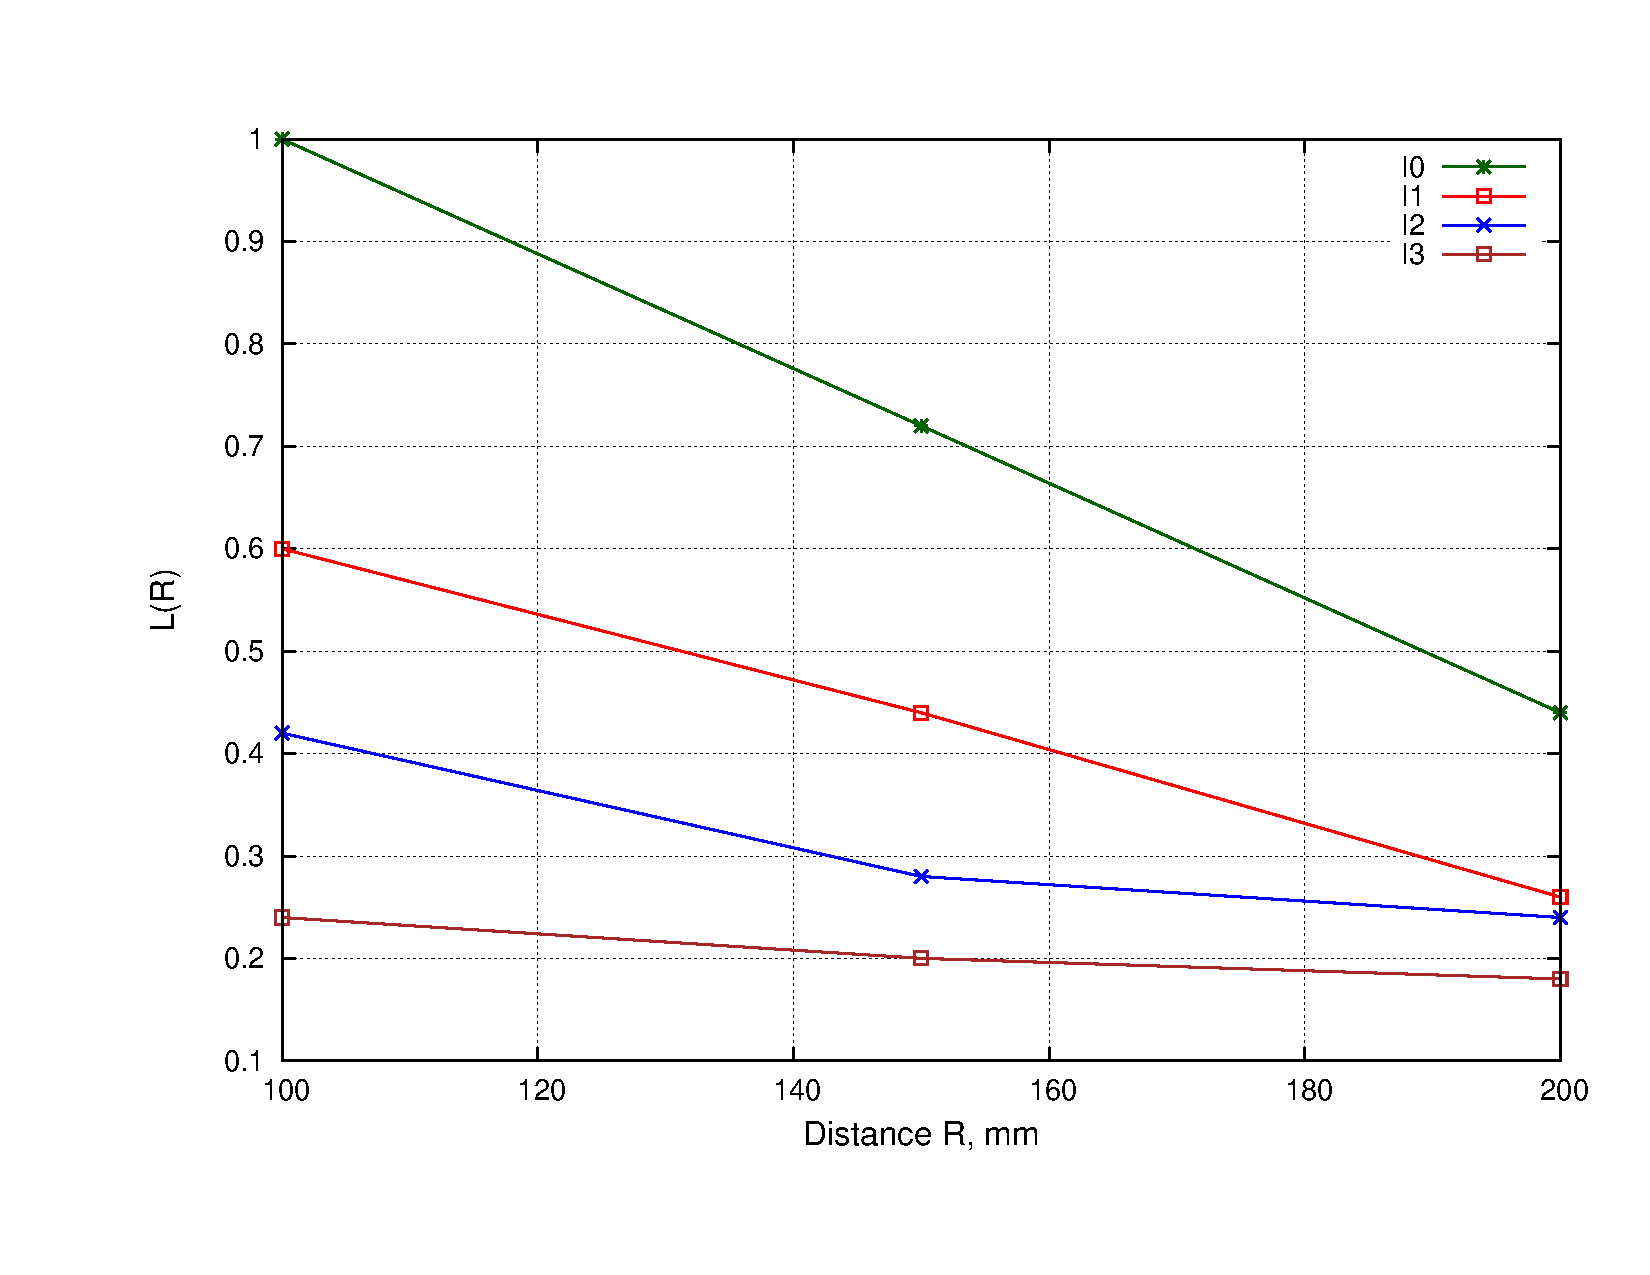
\includegraphics[width = \textwidth]{plot1.pdf}
    \vspace{-30pt}
    \caption{График зависимости величины ЭМП в области геометрической тени от расстояния до цилиндра.}
    \label{fig:plot1}
\end{figure}

\begin{figure}[h!t]
    \centering
    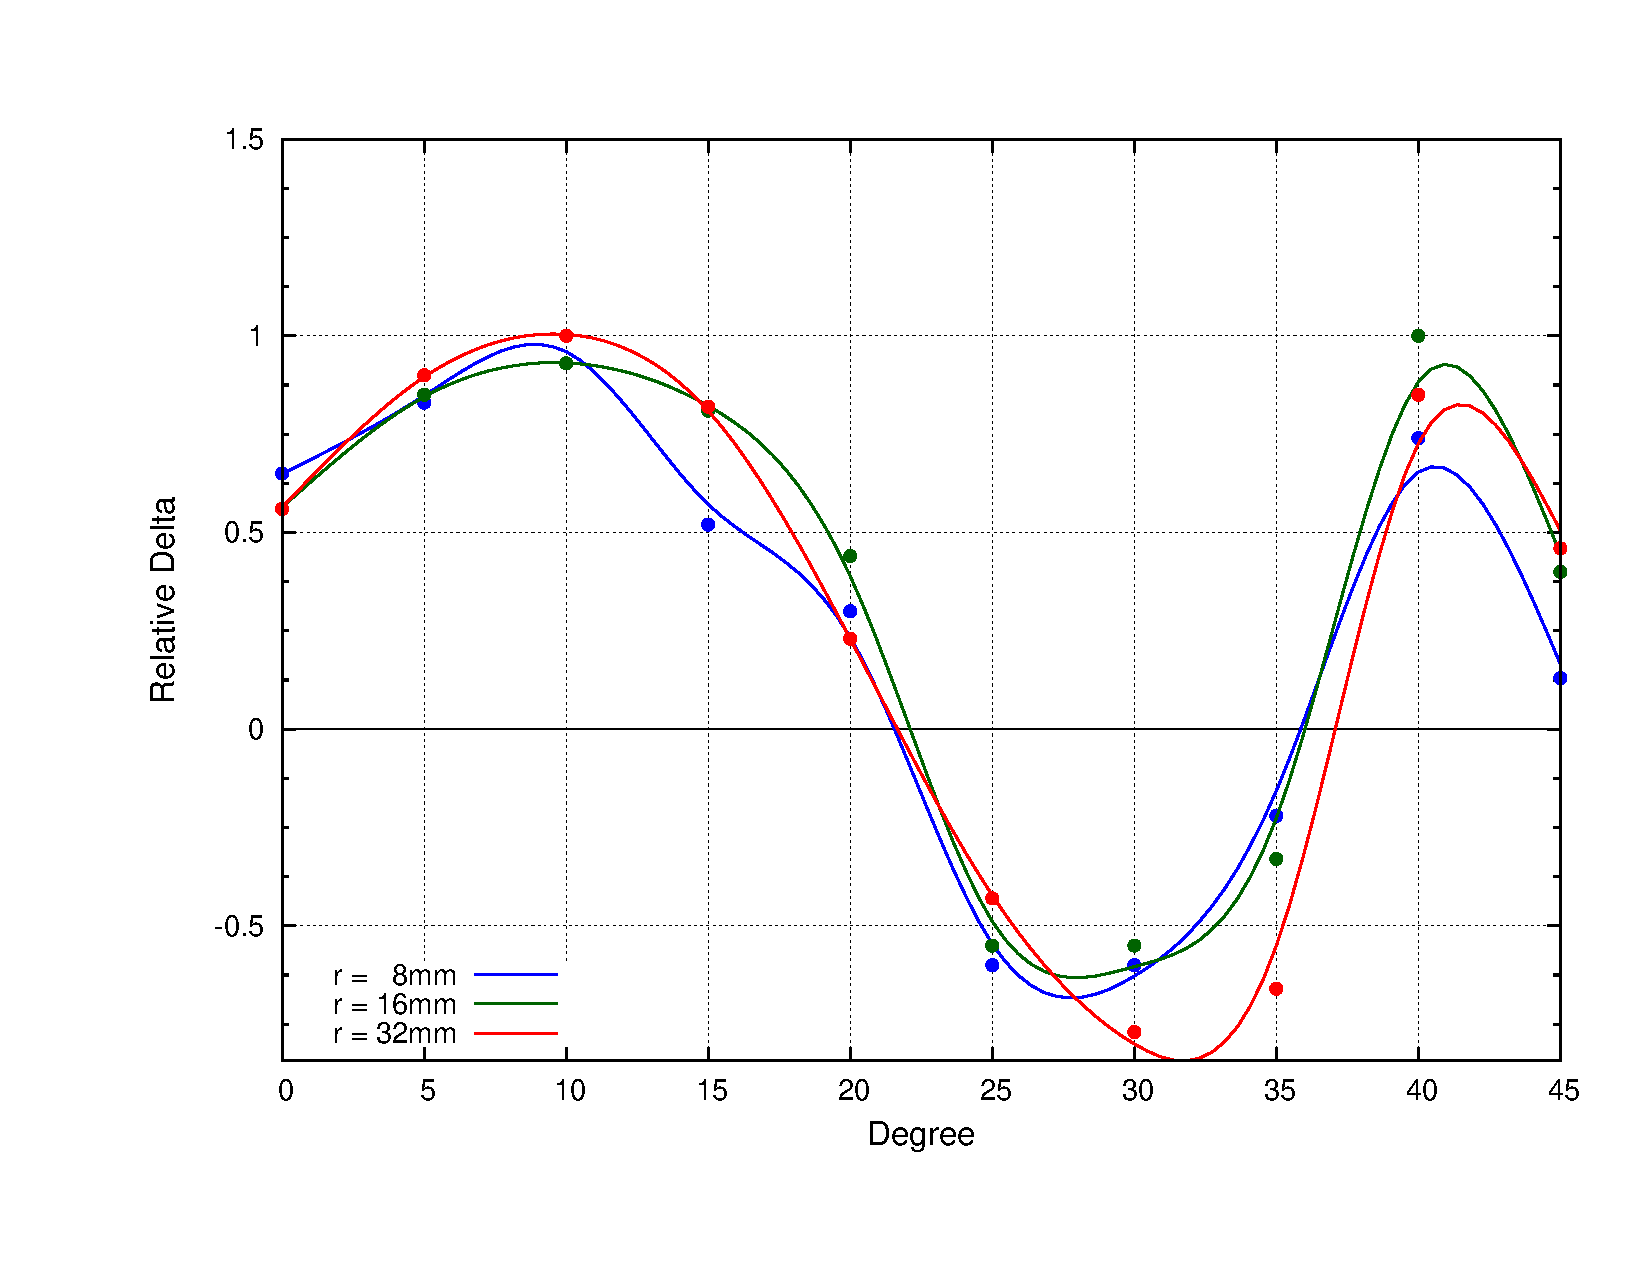
\includegraphics[width = \textwidth]{plot2.pdf}
    \vspace{-30pt}
    \caption{График зависимости величины ЭМП от угла преломления ЭМВ на цилиндре.}
    \label{fig:plot2}
\end{figure}

\begin{figure}[h!t]
    \centering
    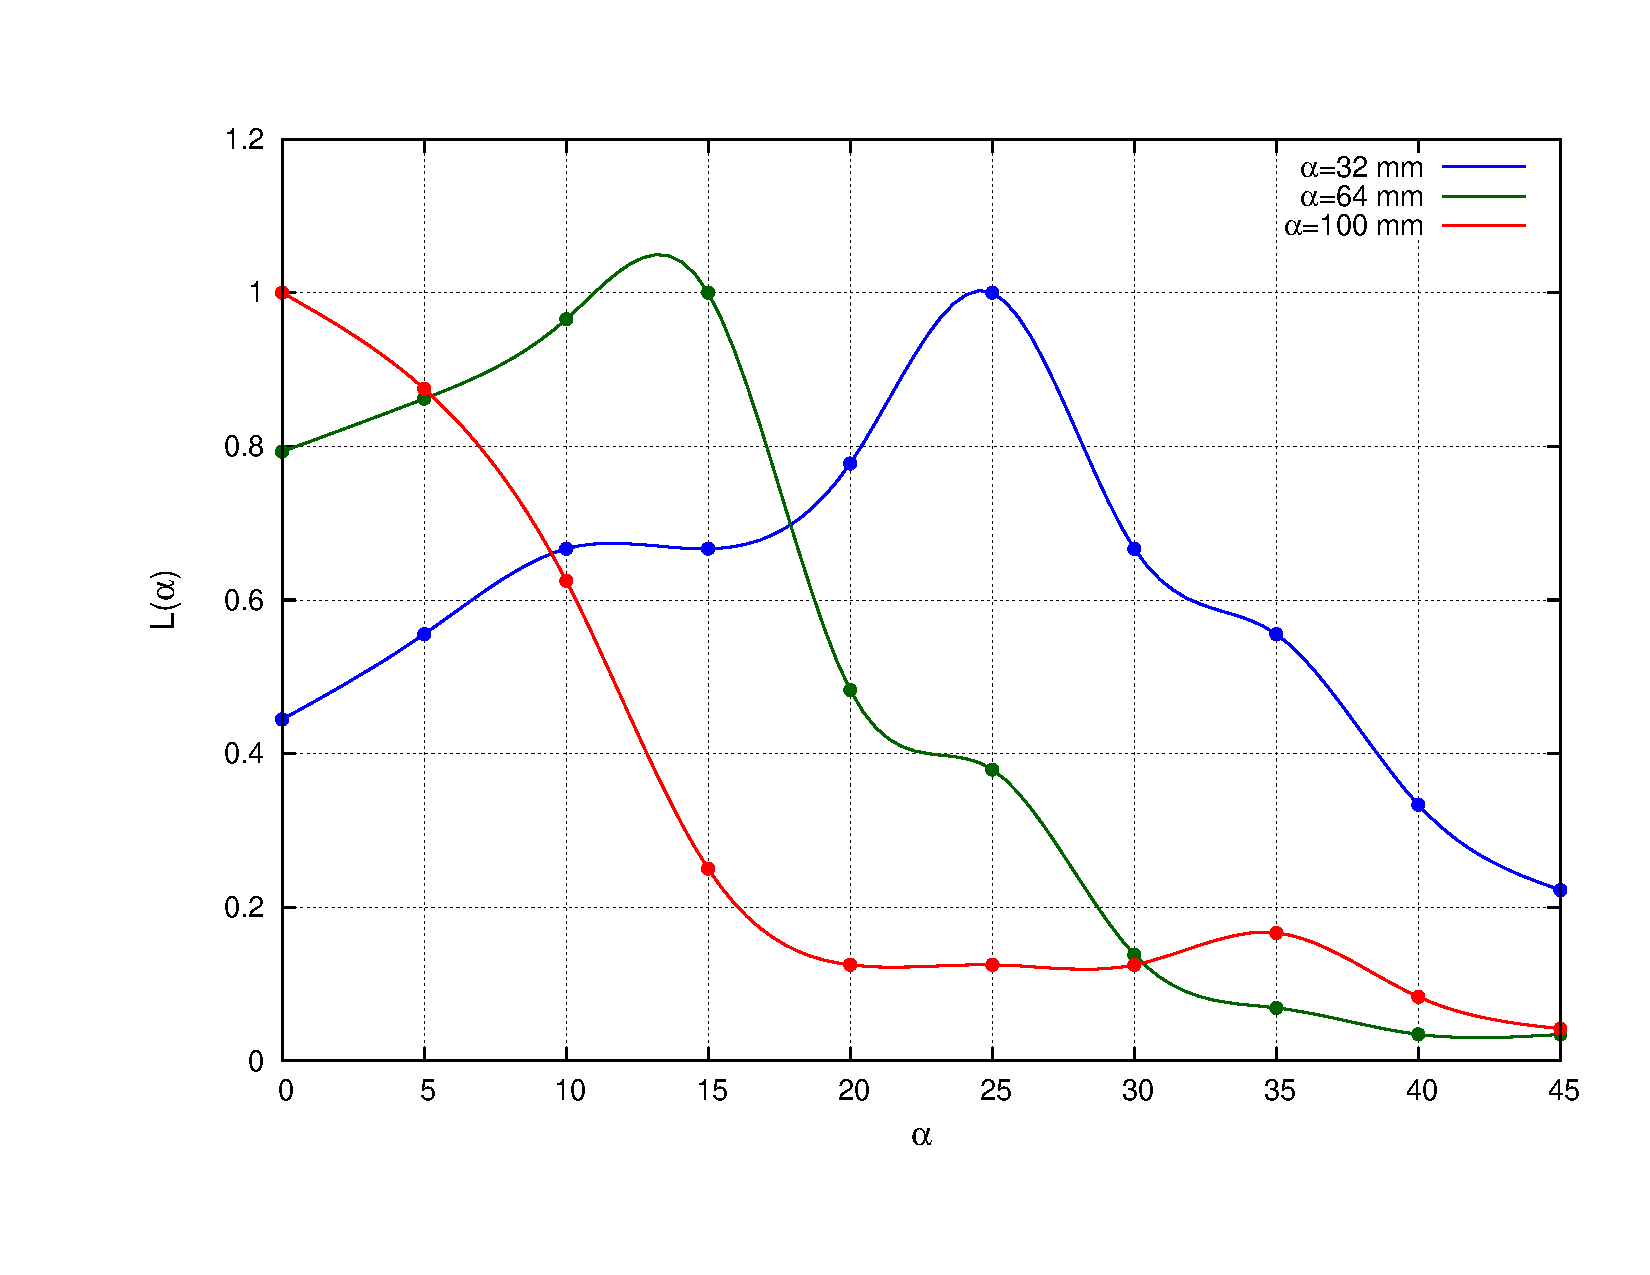
\includegraphics[width = \textwidth]{plot3.pdf}
    \vspace{-30pt}
    \caption{График зависимости величины ЭМП от угла преломления ЭМВ на щели.}
    \label{fig:plot3}
\end{figure}

\begin{figure}[h!t]
    \centering
    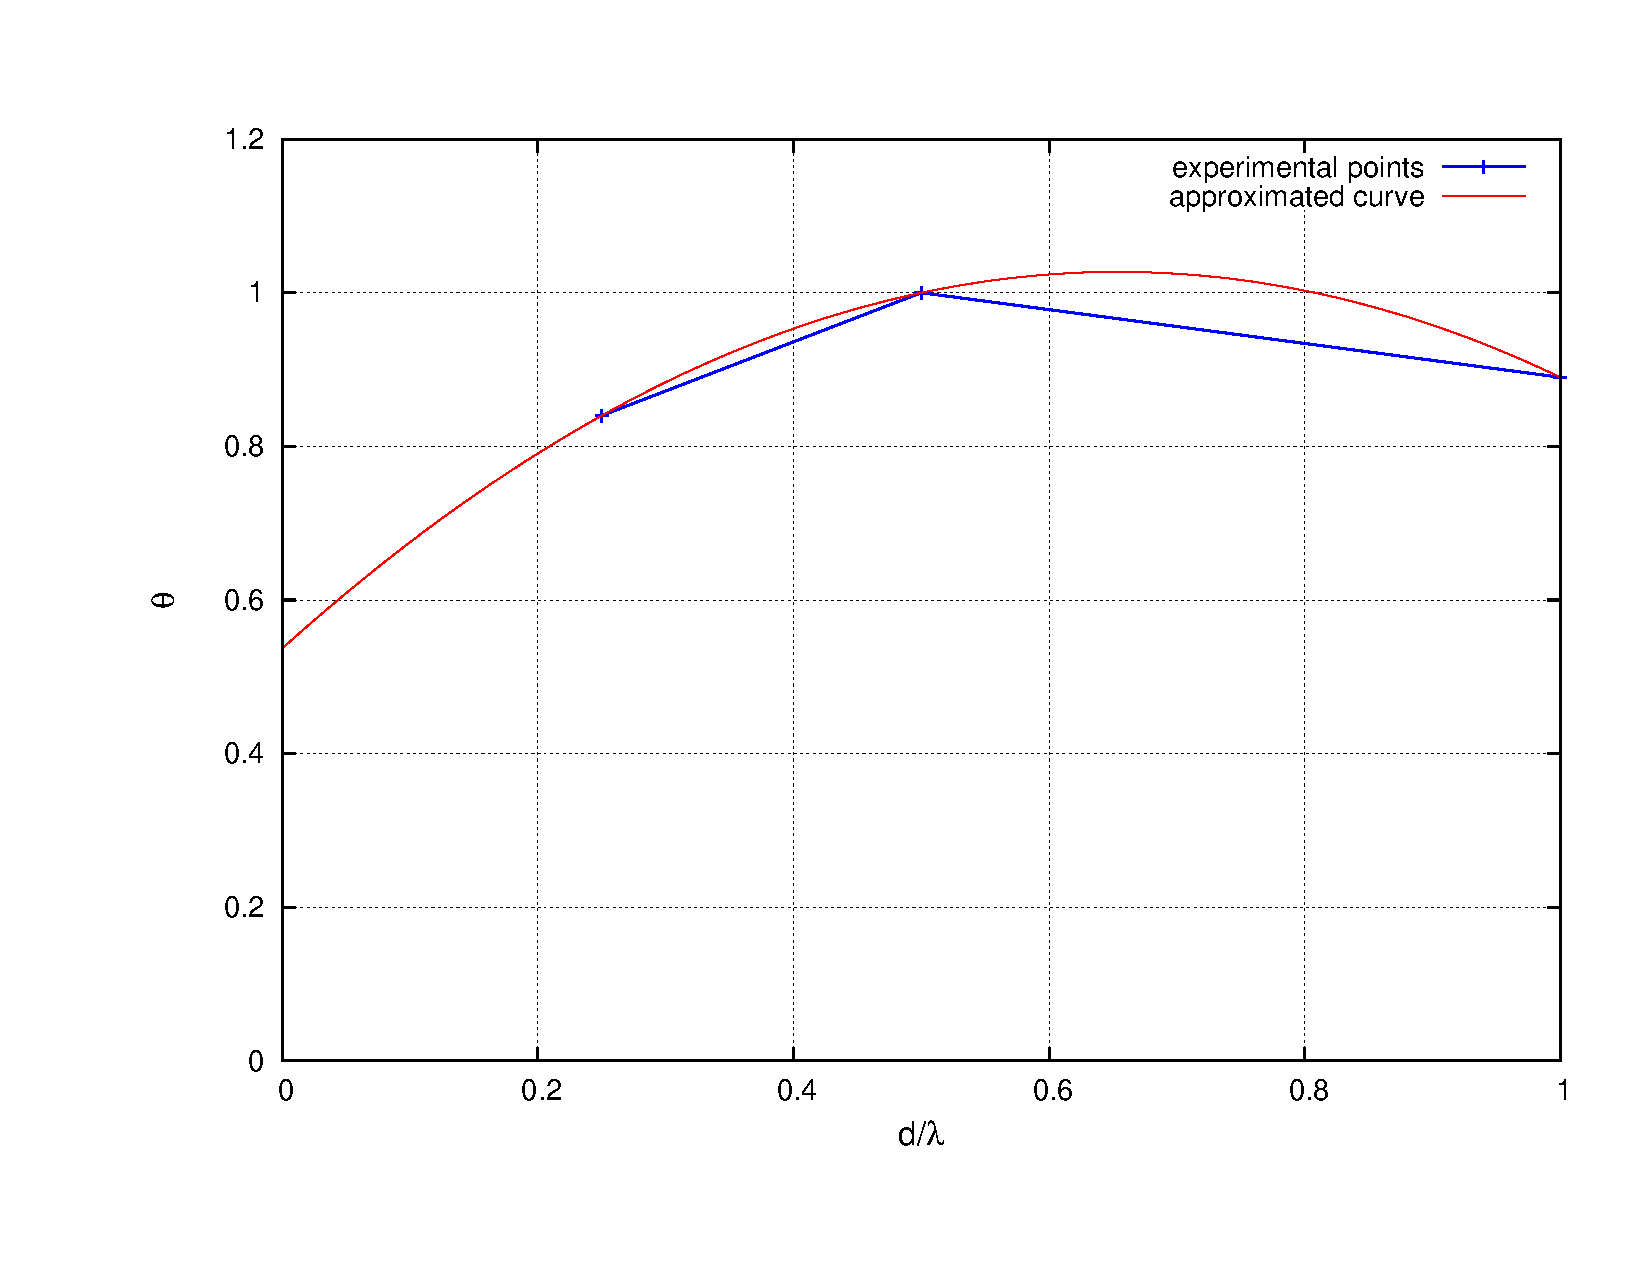
\includegraphics[width = \textwidth]{plot4-1.pdf}
    \vspace{-30pt}
    \caption{График зависимости угла половинной мощности от нормированных размеров цилиндра.}
    \label{fig:plot4}
\end{figure}

\begin{figure}[h!t]
    \centering
    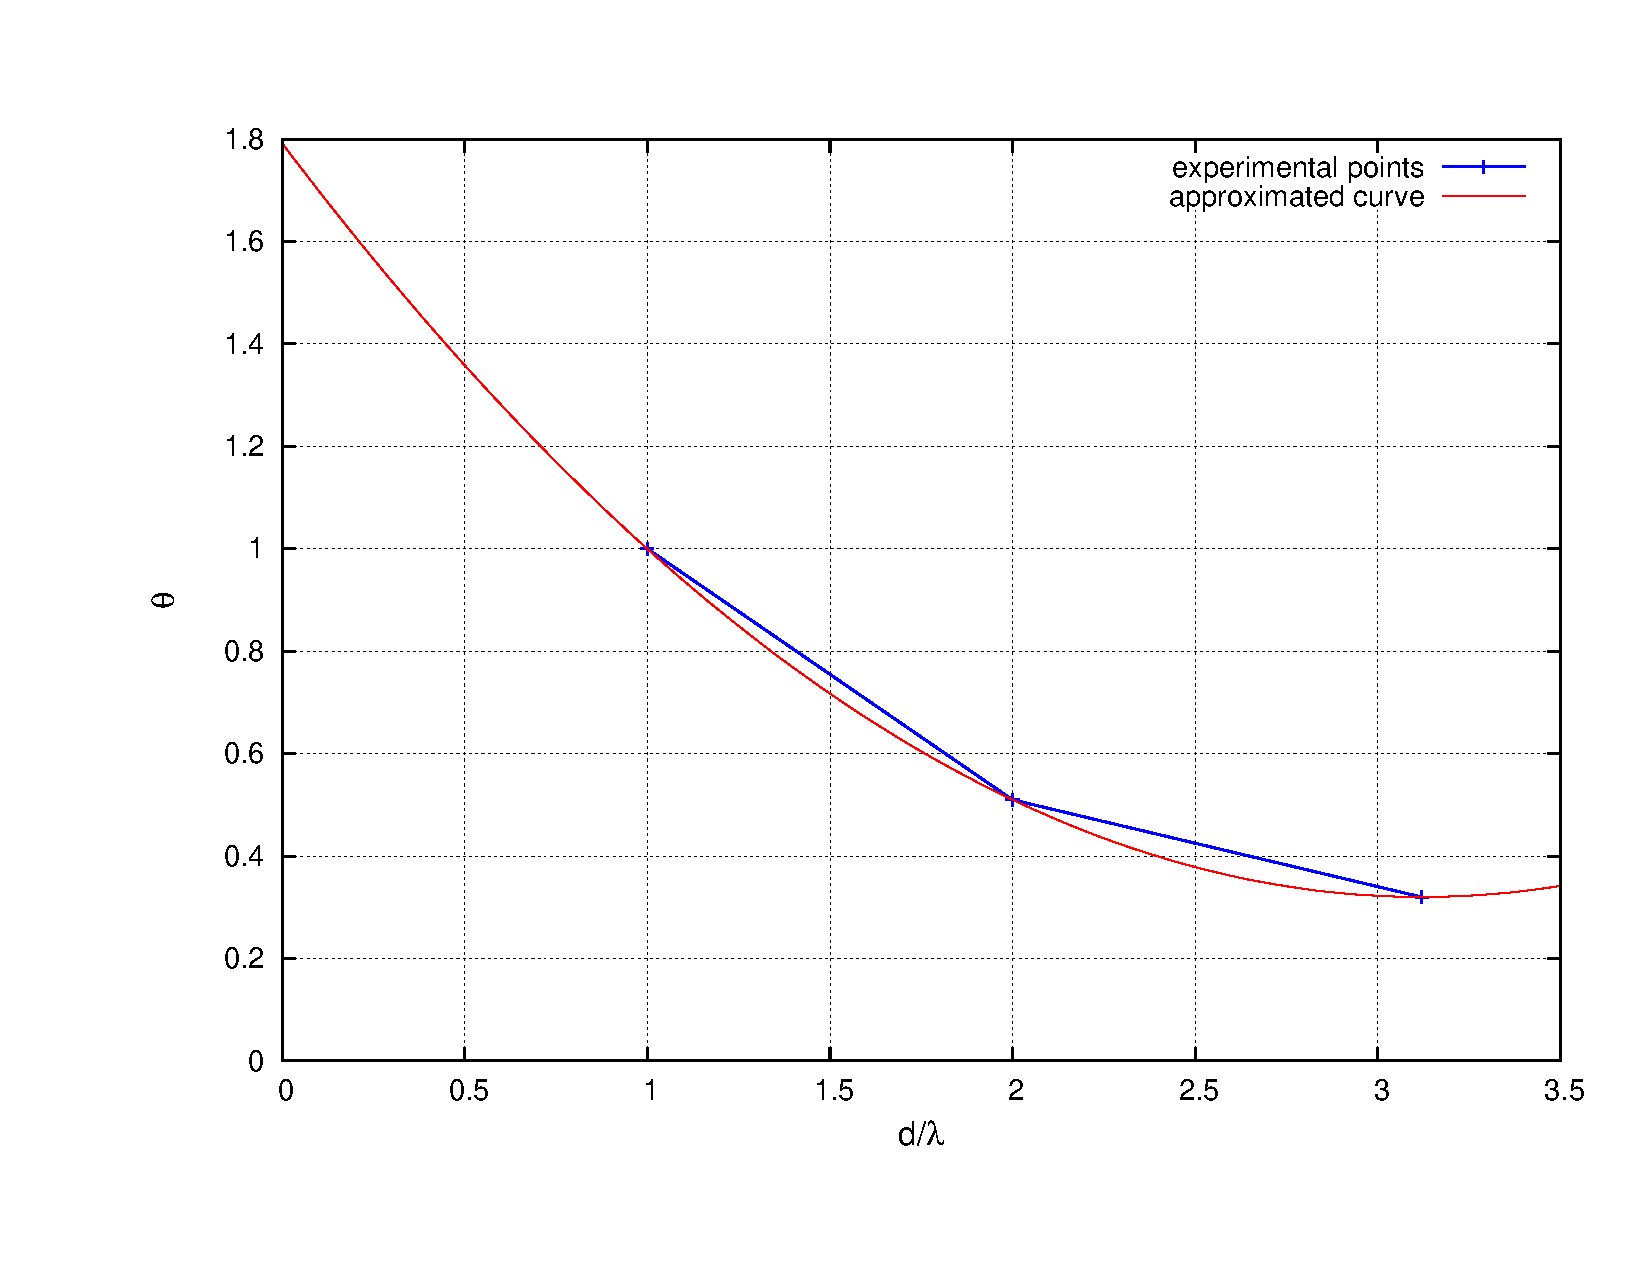
\includegraphics[width = \textwidth]{plot4-2.pdf}
    \vspace{-30pt}
    \caption{График зависимости угла половинной мощности от нормированных размеров щели.}
    \label{fig:plot5}
\end{figure}
\end{document}
